%\chapter{Numerical Examples}
\chapter{SIBM - 避難場所情報ベンチマークツール}

\section{SIBMのコンセプト}
\label{sibm:definition}

SIBM(Shelter Information Benchmark)は避難場所情報と避難作業の関係者に関する情報を中心するデータを生成するツールである.

SIBMは以下の2つの目標に基づいて設計されている:

\begin{enumerate}
  \item
  現実に近いデータの特徴や使用シナリオのこと:災害対策のため、実際の災害にすぐ対応できることはとても大切な目標である.
  \item 拡張性を持つこと:任意の規模を持つデータセットやそのデータの複雑度を選択できることが実験に対する重要な要素であると考えている.
\end{enumerate}

その以外にも、研究分野や使用目的によって、様々な場面で活用できることが考えられる.

\section{データ構成の設計}
\label{sibm:data_structure}

SIBMが2つの情報:避難場所情報、人間(ユーザ)の情報を対象とする.避難場所とユーザのつながりが図\ref{fig:sibm_structrure}のように構成される.

避難場所情報が避難場所の詳細情報を表すものである.その構造は以下のようになる(図\ref{fig:sibm_structrure}):

\begin{itemize}
  \item 地上の座標、住所
  \item 収容人数
  \item 災害分類(地震・津波・火山・洪水・その他・未確定)
  \item 施設の種類
\end{itemize}

ユーザが3つの対象がある:アシスタント、避難者、ボランチア.ユーザ全体に対する基本個人情報が生成され、タイプ別に対する情報が追加される.
例えば、ユーザ全体の情報には、ユーザの氏名・年齢・住所・性別などの情報が持つ.
情報共有範囲を管理するために、各タイプそれぞれに対するアクセス可能範囲の情報が追加される.

\begin{figure}[h!]
 	\begin{center}
 		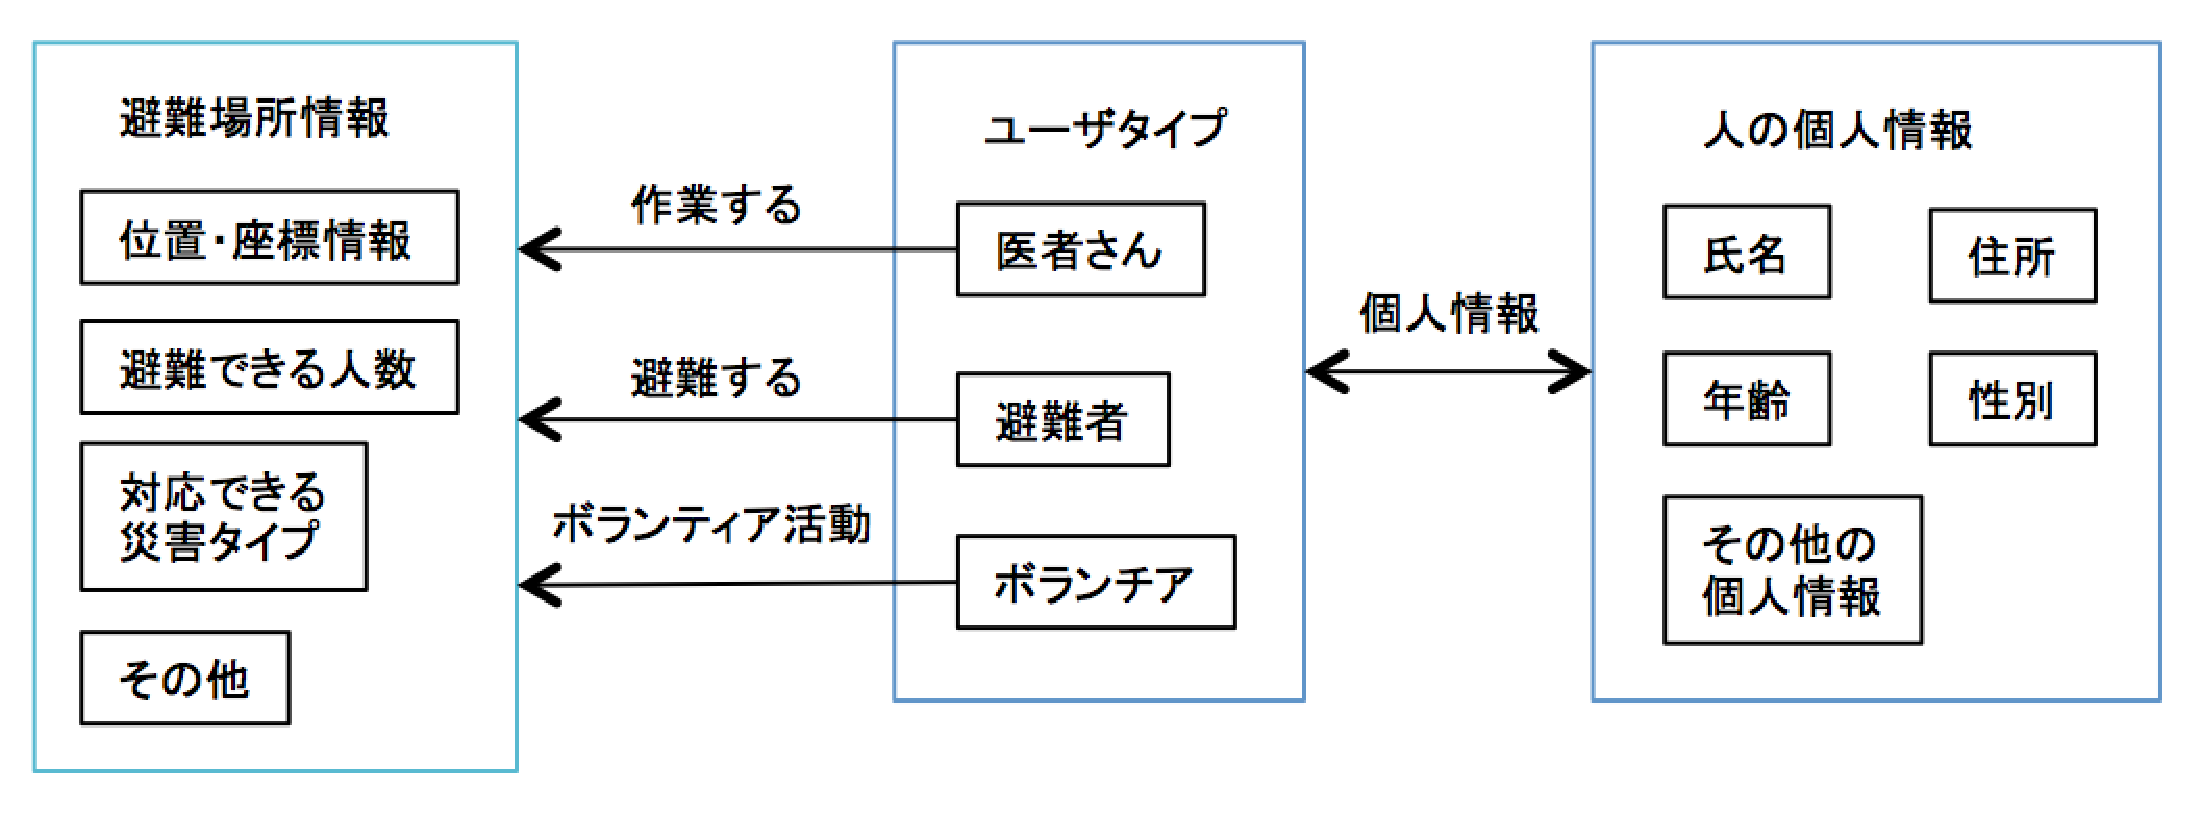
\includegraphics[width=80mm]{./images/fig1.eps}
 		\caption{避難場所データ構成}
 		\label{fig:sibm_structrure}
 	\end{center}
\end{figure}

避難場所情報全体には、避難場所の詳細情報と、その避難場所で避難する・作業する人たちの情報が含まれる.
避難する人や避難場所で作業する人の割合が適切に生成される(図\ref{fig:sibm_shelter}).
また、現実には、災害が発生するとき、一人以上の家族単位で避難することが考えられる.

\begin{figure}[h!]
 	\begin{center}
 		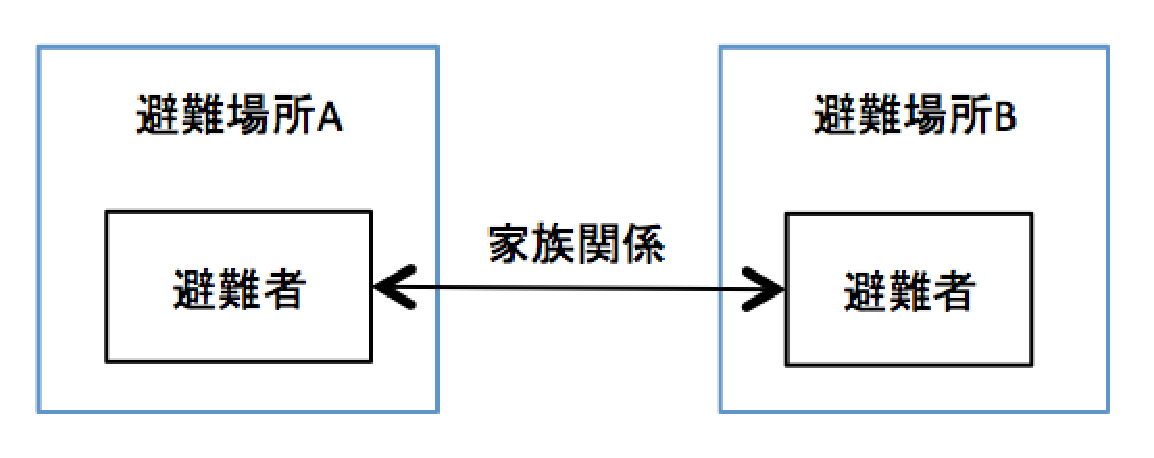
\includegraphics[width=75mm]{./images/fig2.eps}
 		\caption{避難場所全体の構成}
 		\label{fig:sibm_shelter}
 	\end{center}
\end{figure}

また、家族全員が違う避難場所で避難することがある.SIBMでは、そのような関連を追加することが可能である.
図3のように、違う避難場所で避難する人々間の家族関係が生成される.

\begin{figure}[h!]
 	\begin{center}
 		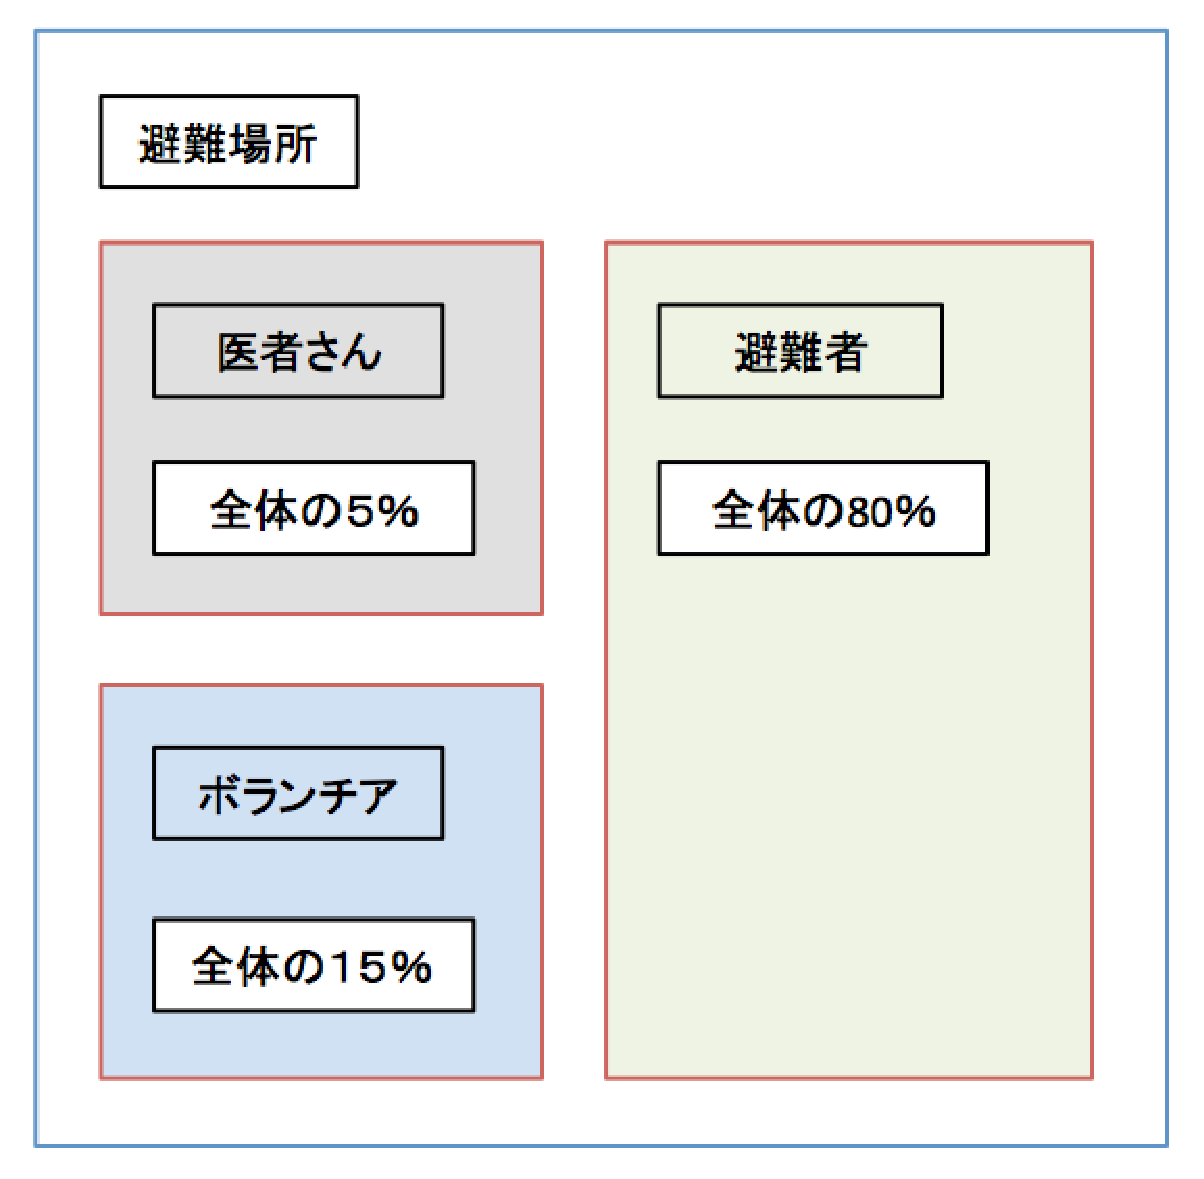
\includegraphics[width=70mm]{./images/fig4.eps}
 		\caption{家族関係}
 		\label{fig:sibm_relationship}
 	\end{center}
\end{figure}

最後に、現実のように避難場所が都道府県単位で管理することを表す.
本稿では、平成24年度国土交通省による公開された全国47都道府県の避難場所情報(役12.5万箇所)を使用した.

\begin{figure}[h!]
 	\begin{center}
 		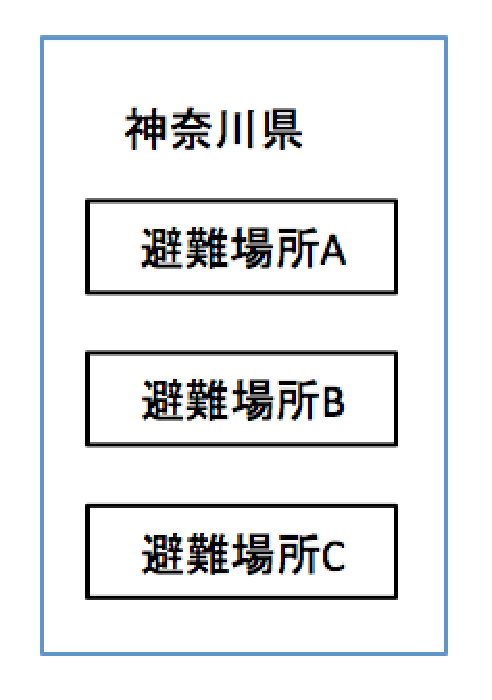
\includegraphics[width=35mm]{./images/fig3.eps}
 		\caption{都道府県単位の避難場所構成}
 		\label{fig:sibm_prefecture}
 	\end{center}
\end{figure}

\section{データクラスの定義}

SIBMでは、入力したパラメーターによる、データセットの規模や情報の複雑度を適切に生成される.
データが生成される際、データ各種を部分的に生成され、最後に設定したパラメーターを導入して、結果を出力する.

関係者情報クラスの詳細設計が、図\ref{fig:sibm_class_person}のようになる.

\begin{figure}[h!]
 	\begin{center}
 		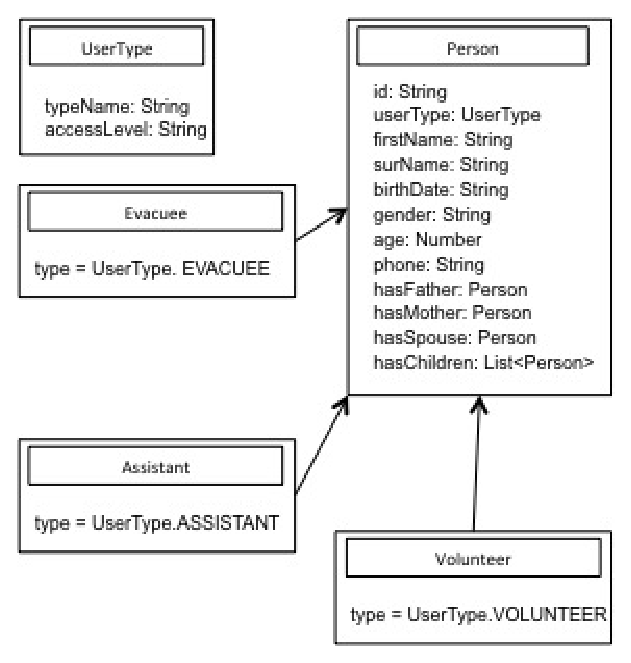
\includegraphics[width=75mm]{./images/class_person.eps}
 		\caption{関係者クラス図}
 		\label{fig:sibm_class_person}
 	\end{center}
\end{figure}

共有となるクラス:\textbf{Personクラス}と\textbf{UserTypeクラス}がある.

\begin{itemize}
  \item \textbf{Personクラス}が、関係者の一般的な情報を持ち、それぞれに対するフィルドを定義する.
  \item \textbf{UserTypeクラス}が関係者の種類を分ける情報とその種類に対するアクセスレベルを持つ.
\end{itemize}

関係者クラスを定義する時、そのクラスが\textbf{Personクラス}を継承する.そして、そのクラスの種類を定義する\textbf{UserType}クラスの確定インスタンスを持つことになる.
図\ref{fig:sibm_class_person}のように、避難者(\textbf{Evacueeクラス})、アシスタント(\textbf{Assistantクラス})、ボランティア(\textbf{Volunteerクラス})
が定義される.

避難場所情報が図\ref{fig:sibm_class_shelter}のように、\ref{sibm:data_structure}に設計したデータ構成を実装したクラス図である.

\begin{figure}[h!]
 	\begin{center}
 		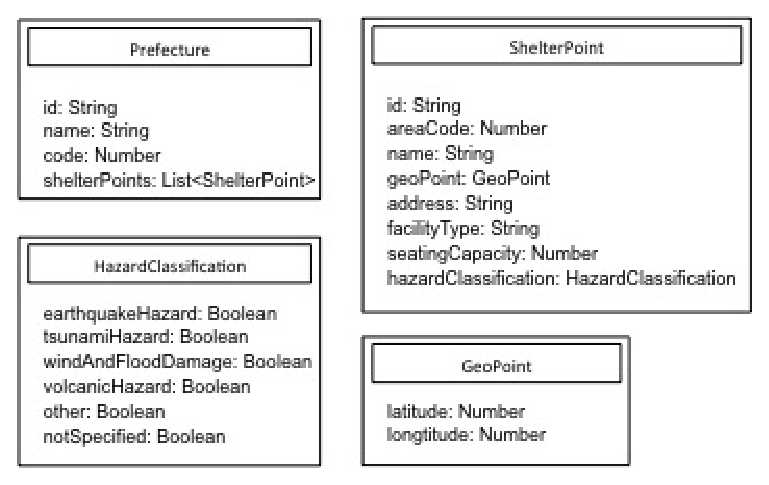
\includegraphics[width=80mm]{./images/class_shelter.eps}
 		\caption{避難場所クラス図}
 		\label{fig:sibm_class_shelter}
 	\end{center}
\end{figure}

\begin{itemize}
  \item \textbf{GeoPointクラス}が、避難場所の地上位置を定義するクラス.実際に、避難場所の位置検索などに使用されることがある.
  \item
  \textbf{HazardClassificationクラス}が、特定の避難場所が対応できる災害のタイプを定義するクラス.
  \textbf{true}か\textbf{false}値を持ち、避難できるかできないかの意味を持つ.
  SIBMでは、6つの災害タイプを対象とする:地震・津波・火山・洪水・その他・未確定.
  \item \textbf{ShelterPointクラス}が、避難場所の一つを定義するクラスである.
  \item \textbf{Prefectureクラス}が、都道府県の情報とそこにある避難場所の情報を定義するクラスである.
\end{itemize}

\section{情報リソース}
\label{sibm:resource}

SIBMでは、現実に近い情報を生成する目的を持つ.その目的を実装するために、実際にある情報元を使用することと、実際に近い情報を生成するツールを使用した.
SIBMが使用する避難場所情報では、自然災害発生時に住民を避難させ、又は避難住民等の救援を行うための施設で、市町村長が指定し地域防災計画等に掲載されている施設
(ただし、最新の情報ではない場合もあることから、災害時に避難施設を利用できることにならない).
SIBMが生成する人間の個人情報は、実際の人間の個人情報ではないが、実際に近い情報を生成する目標がある.上記の実装を行うためのリソースは以下のように説明する.

\begin{itemize}
	\item
	\textbf{国土交通省}(MLIT\footnote{Ministry of Land, Infrastructure, Transport and
	Tourism}) による提供した避難施設情報\footnote{http://nlftp.mlit.go.jp/ksj/index.html}.
	SIBMが生成する避難場所情報がMLITによる提供した避難施設情報を使用することになった.その情報の特徴が(表\ref{table:data_shelter})からわかる.
	
	\begin{table}[h]
	\begin{center}
	\begin{tabular}{| l | l | l | p{48mm} |}
		\hline
		\rowstyle{\bfseries}
		データ項目 & フォーマット & 整備年度 & 内容 \\
		\hline
		避難施設 & 点 & 平成24年度 & 位置、行政区域、名称、住所、施設の種類、収容人数、施設規模、災害分類 \\
		\hline
	\end{tabular}
	\caption{避難場所情報の詳細}
	\label{table:data_shelter}
	\end{center}
	\end{table}

	\item 人間の情報では、\textbf{Random profile web
	API
	(RPA)}\footnote{http://randomprofile.com/api-for-developers}を参考にしたツールを作成して使用する.RPAで生成した個人情報は
	表\ref{table:data_person}のようになる.しかし、RPAでは、使用制限があるため、SIBMがそのモデルを参考にして人間個人情報を生成するツールを構成する.
	構成したツールを使用して人間の個人情報を生成することができ、さらに複雑な情報(家族関係など)を生成することも可能である.
	
	\begin{table}[h]
	\begin{center}
	\begin{tabular}{| l | p{72mm} |}
		\hline
		\rowstyle{\bfseries}
		フィルド & 値 \\
		\hline
		ユーザID & 54b0ae57a0dcc \\
		\hline
		firstName & 心 \\
		\hline
		surname & 真塩 \\
		\hline
		translitFirstName & Kokoro \\
		\hline
		translitSurname & Mashio \\
		\hline
		gender & Female \\
		\hline
		birthday & 1993-09-01 \\
		\hline
		age & 21 \\
		\hline
		country & Japan \\
		\hline
		passportNumber & TX1338642 \\
		\hline
		phone & +8152-324-1820 \\
		\hline
		address & 452-1179, Kawazoe, Shiraoi-cho Shiraoi-gun, Hokkaido \\
		\hline
		email & Kokoro.Mashio@e4xample.com \\
		\hline
		occupation & Animal Control Worker \\
		\hline
	\end{tabular}
	\caption{個人情報の例}
	\label{table:data_person}
	\end{center}
	\end{table}
\end{itemize}
